\chapter{直流稳压电源}
\Par 将交流电转换成直流电一共需要四步:变压、整流、滤波、稳压.
\begin{figure}[htbp]
	\centering
	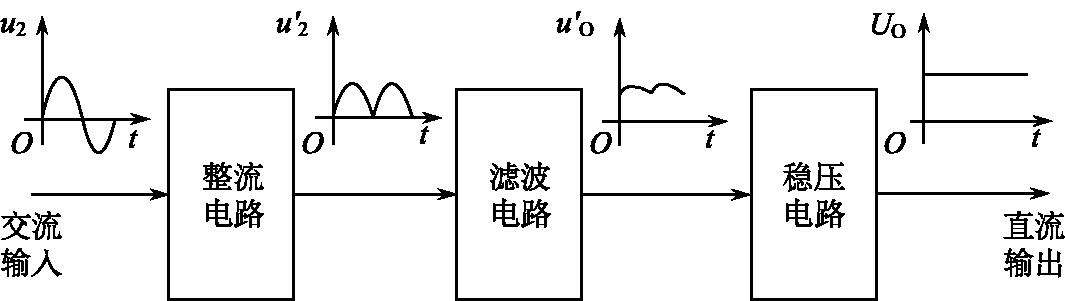
\includegraphics[width=0.65\textwidth]{直流稳压电源的原理.jpg}
	\caption{直流稳压电源的原理}
	\label{fig:直流稳压电源的原理}
\end{figure}

\section{\K 整流电路}

\Par 整流电路的种类较多,按交流电源的相数可分为单相和多相整流电路;按流过负载的电流波形可分为半波和全波整流电路.

\Par 我们只介绍单相整流电路.对于单相半波整流电路,我们很容易明白它的原理.
\begin{figure}[htbp]
	\centering
	\begin{minipage}[b]{0.48\textwidth}
        \centering
        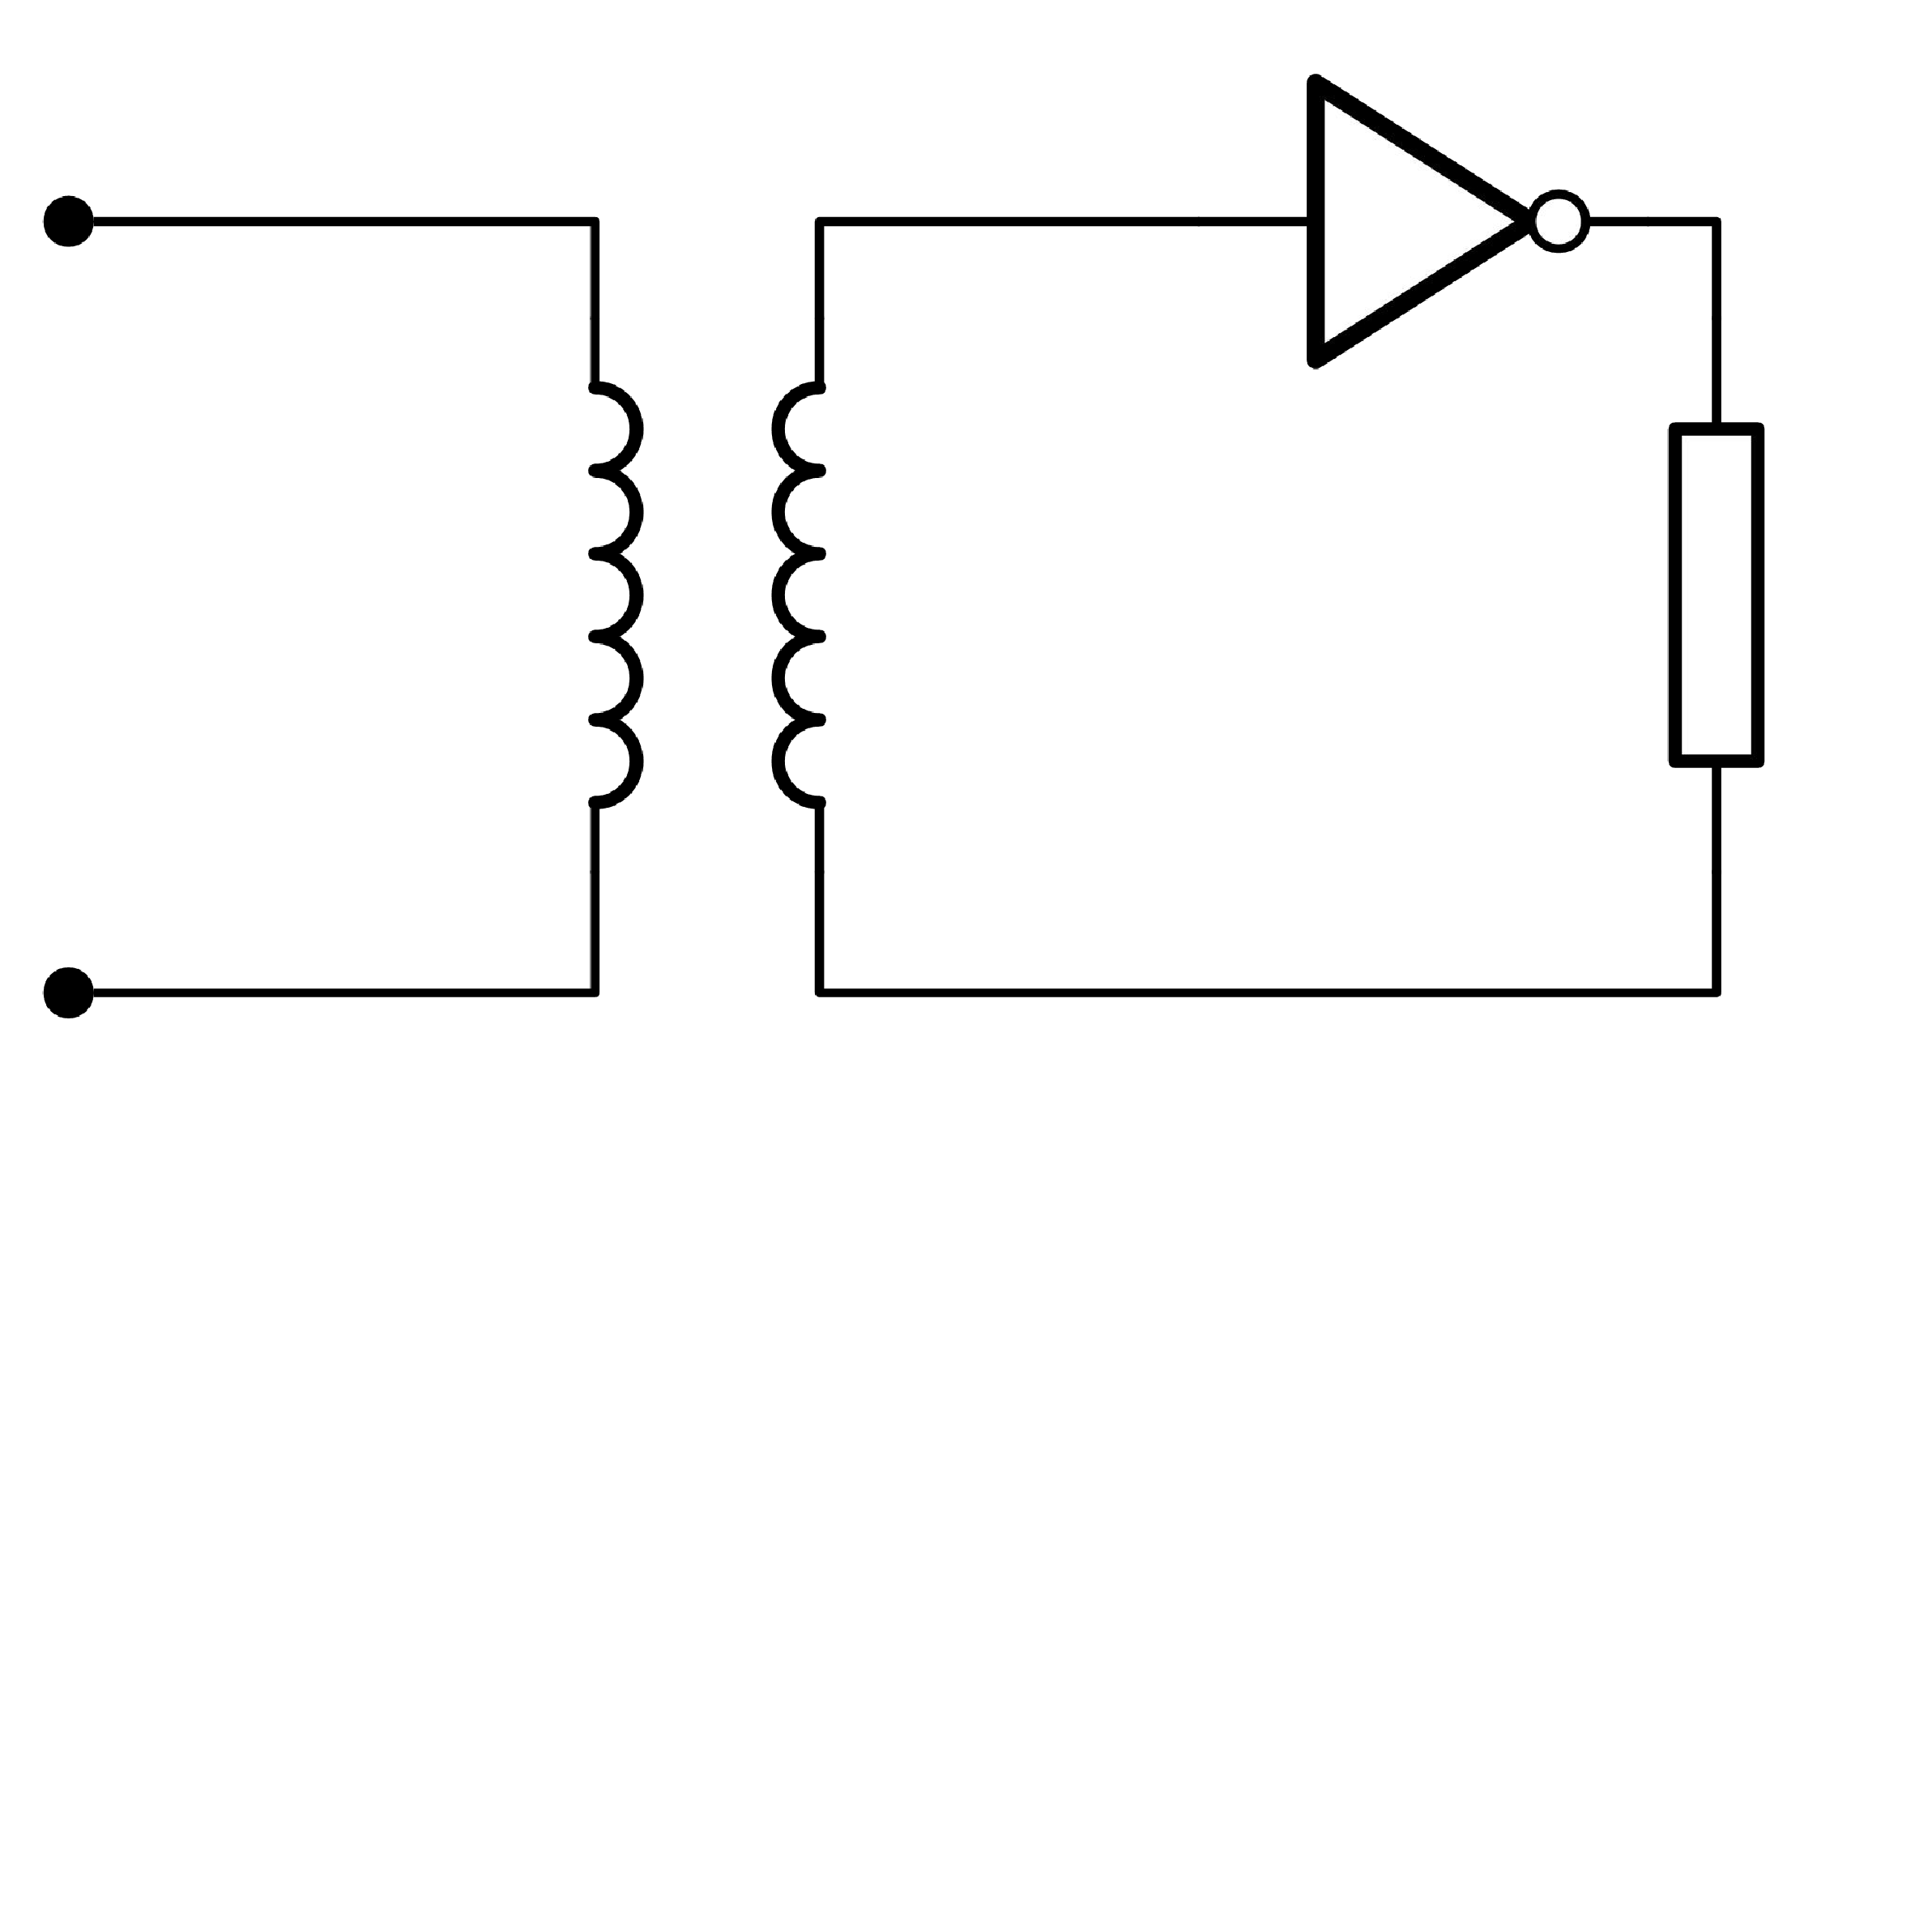
\includegraphics[width=0.85\textwidth]{单相半波整流电路.pdf}
        \caption{单相半波整流电路}
        \label{fig:单相半波整流电路}
    \end{minipage}
    \begin{minipage}[b]{0.48\textwidth}
        \centering
        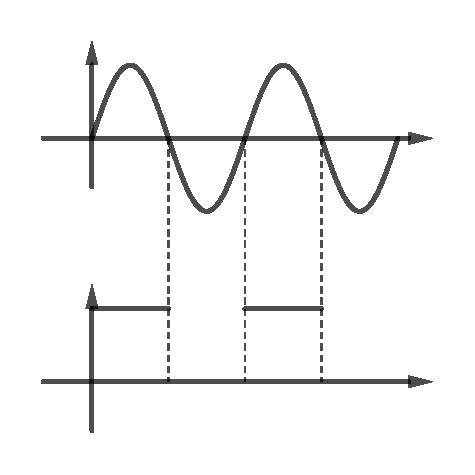
\includegraphics[width=0.85\textwidth]{单相半波整流电路特性曲线.pdf}
        \caption{单相半波整流电路特性曲线}
        \label{fig:单相半波整流电路特性曲线}
    \end{minipage}
\end{figure}

\Par 下面重点说明单相全波整流电路,由于画图困难,隧只在一张图上讲解.如图\ref{fig:单相桥式整流电路}所示,当输入的电压是上正下负的时候,可以知道$D_1$与$D_4$相交的节点是电位最高点,而$D_2$与$D_3$相交的节点是电位最低点,因此二极管$D_1$导通,视为导线.此时,$D_2$上端为高点位,下端为低电位,因此它截止.同理,$D_4$也将截止,而$D_3$导通.从而形成了电流依次流经$D_1$、$R_L$和$D_3$的电路,此时$R_L$上正下负.

\begin{figure}[htbp]
	\centering
	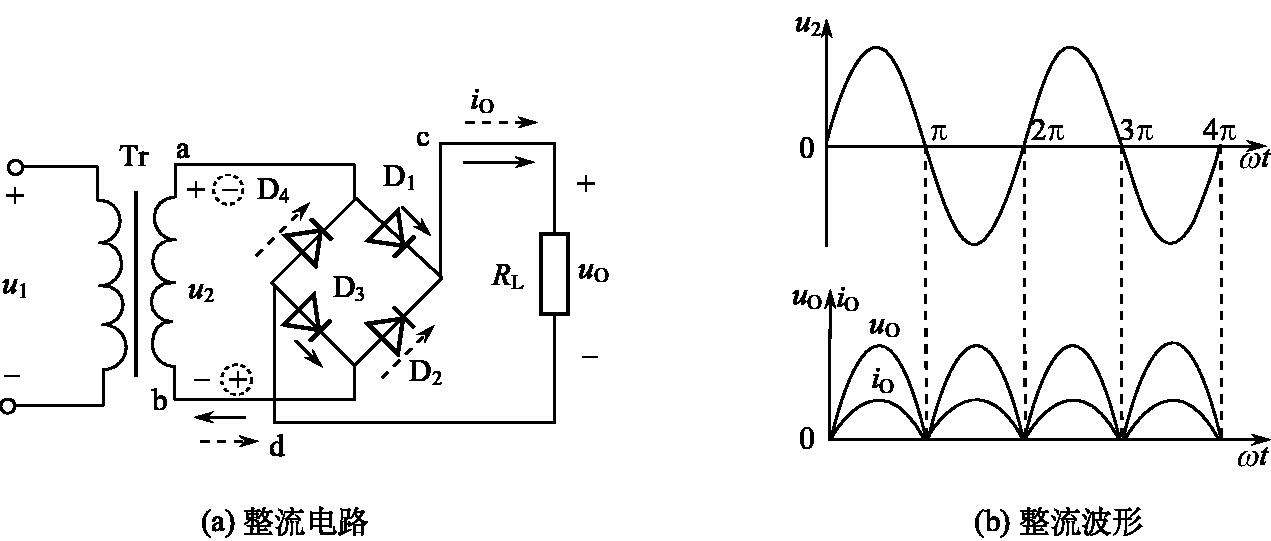
\includegraphics[width=0.65\textwidth]{单相桥式整流电路.jpg}
	\caption{单相桥式整流电路}
	\label{fig:单相桥式整流电路}
\end{figure}

\Par 同理,对于下正上负的输入电压有同样的分析,此时,$D_2$和$D_4$导通,$D_1$和$D_3$截止,从而形成了电流依次流经$D_2$、$R_L$和$D_4$的电路,$R_L$同样上正下负.

\Par 为了了解输出的整流电压的性质,我们需要知道整流电压的参数(设输入电压为$u=\sqrt{2}U_2\sin \omega t$):
\begin{enumerate}[(1)]
    \item 整流电压平均值$U_o$
    \begin{equation}
        U_o=\frac{2}{T}\int_0^{T/2}{\sqrt{2}U_2\sin \omega t\mathrm{d}t}\approx 0.9U_2
    \end{equation}
    \item 整流电流平均值$I_o$
    \begin{equation}
        I_o=\frac{U_o}{R_L}=0.9\frac{U_2}{R_L}
    \end{equation}
    \item 每管电流平均值$I_D$
    \begin{equation}
        I_D=\frac{1}{2}I_o=0.45\frac{U_2}{R_L}
    \end{equation}
    \item 每管承受的最高反向电压$U_{DRM}$
    \begin{equation}
        U_{DRM}=\sqrt{2}U_2
    \end{equation}
    \item 变压器副边电流有效值$I_2$
    \begin{equation}
        I_o=\frac{2}{T}\int_0^{T/2}{\sqrt{2}I_2\sin \omega t\mathrm{d}t}\approx 0.9I_2\Longrightarrow I_2\approx 1.1I_o
    \end{equation}
\end{enumerate}

\Par 通常我们用一个整流桥(硅桥堆)来代替四个二极管拼成的单相桥式整流电路,它就相当于一个黑箱.





\section{\K 滤波电路}
\Par 由于滤波电路的内容比较简单,我们这里就只以桥式滤波电路为例.如图\ref{fig:电桥滤波电路}所示,刚接上电源的时候,电容和负载$R_L$两端接正向整流电压,电容处于充电状态.

\begin{figure}[htbp]
	\centering
	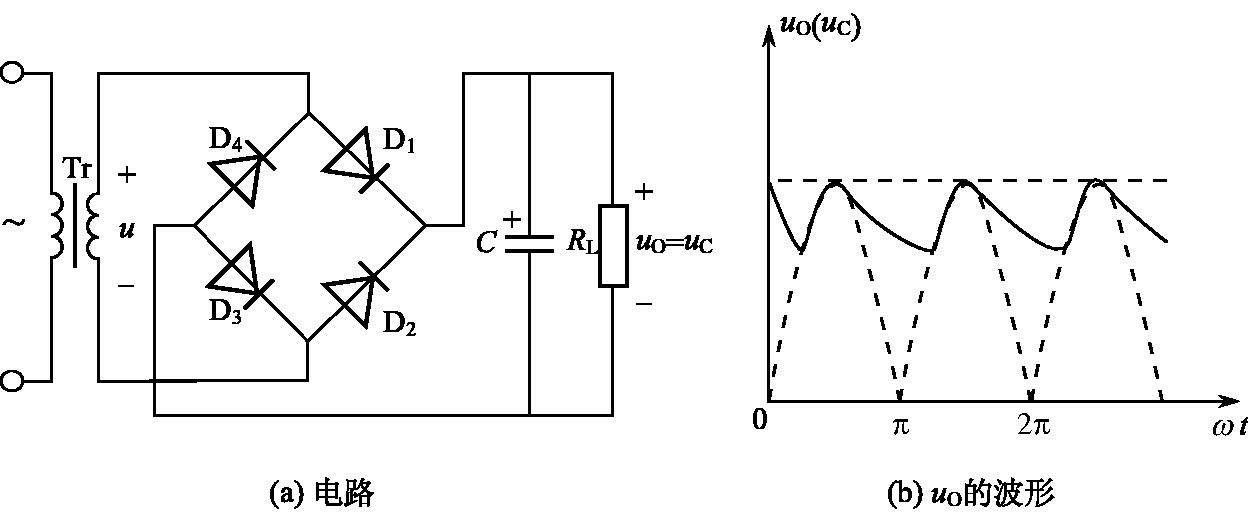
\includegraphics[width=0.55\textwidth]{电桥滤波电路.jpg}
	\caption{电桥滤波电路}
	\label{fig:电桥滤波电路}
\end{figure}

\Par 当电压达到峰值开始下降的时候,电容开始放电.由于电容的放电满足暂态过程,呈指数减小,而整流电压减小的更快,因此电容会维持着$R_L$两端电压让它的减小放缓.

\Par 直到整流电压升高到与电容电压相等,并进一步上升时,电容又开始充电,由此构成了一个循环.

\Par 由上面的分析我们可以知道,电容放电的暂态过程越慢,对我们滤波越有利,因此我们应当选择时间常数$\tau =R_LC$大的电容,通常我们要求
\begin{equation}
    \tau =R_LC\ge 3\sim 5\left( \frac{T}{2} \right) 
\end{equation}

\section{\K 稳压电路}
\subsection{\K 稳压二极管稳压}
\Par 如图\ref{fig:稳压二极管稳压}所示,我们可以选取稳压二极管稳压,而选取的稳压二极管参数一般为
\begin{equation*}
    \begin{cases}
        U_Z=U_O\\
        U_1=2\sim 3U_O\\
        I_{ZM}=1.5\sim 3I_{OM}\\
    \end{cases}
\end{equation*}

\begin{figure}[htbp]
	\centering
	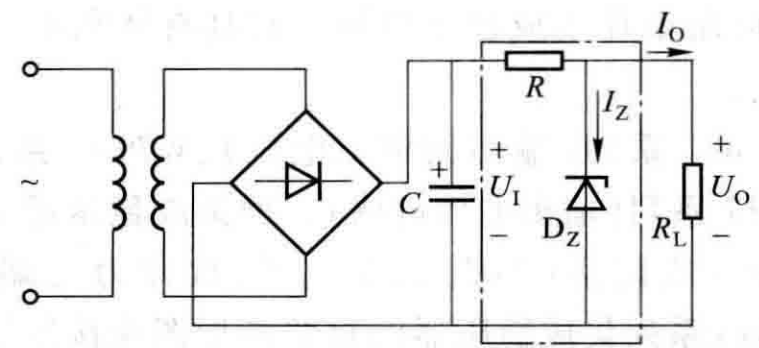
\includegraphics[width=0.45\textwidth]{稳压二极管稳压.png}
	\caption{稳压二极管稳压}
	\label{fig:稳压二极管稳压}
\end{figure}

但是稳压二极管稳压是有缺陷的,一方面它的稳压电压是无法改变的,另一方面,它要求负载电路的电压与它的稳压电压相差不大,因此我们还需要更好的选择.

\subsection{\K 集成稳压电源}
\Par 我们介绍三种集成稳压电源:
\begin{enumerate}[ ]
    \item W78XX系列:输出固定正电压;
    \item W79XX系列:输出固定负电压;
    \item W117/217/317系列:输出可变电压.
\end{enumerate}
\begin{figure}[htbp]
	\centering
	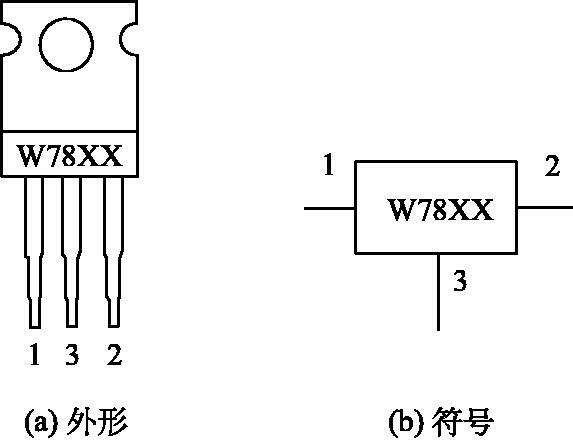
\includegraphics[width=0.35\textwidth]{集成稳压电源.jpg}
	\caption{集成稳压电源}
	\label{fig:集成稳压电源}
\end{figure}

\Par 如图\ref{fig:集成稳压电源}所示,集成稳压电源有三个引脚,分别标记为1、2、3,对于塑料封装的W78XX系列集成稳压电源来说,1输入,2接地,3输出;对于塑料封装的W79XX系列集成稳压电源来说,1接地,2输入,3输出.至于金属封装,可以见下图.
\begin{equation*}
    \begin{array}{l}
        \text{塑料W}78\text{XX系列}\begin{cases}
        {\color[RGB]{0, 0, 240} 1\text{输入}}\\
        2\text{接地}\\
        {\color[RGB]{240, 0, 0} 3\text{输出}}\\
    \end{cases}\Longleftrightarrow \text{金属W}78\text{XX系列}\begin{cases}
        {\color{blue} 1\text{输入}}\\
        {\color[RGB]{240, 0, 0} 2\text{输出}}\\
        3\text{接地}\\
    \end{cases}\\
        \text{塑料W}79\text{XX系列}\begin{cases}
        1\text{接地}\\
        {\color[RGB]{0, 0, 240} 2\text{输入}}\\
        {\color[RGB]{240, 0, 0} 3\text{输出}}\\
    \end{cases}\Longleftrightarrow \text{金属W}79\text{XX系列}\begin{cases}
        1\text{接地}\\
        {\color[RGB]{240, 0, 0} 2\text{输出}}\\
        {\color[RGB]{0, 0, 240} 3\text{输入}}\\
    \end{cases}\\
    \end{array}
\end{equation*}
\begin{figure}[htbp]
	\centering
	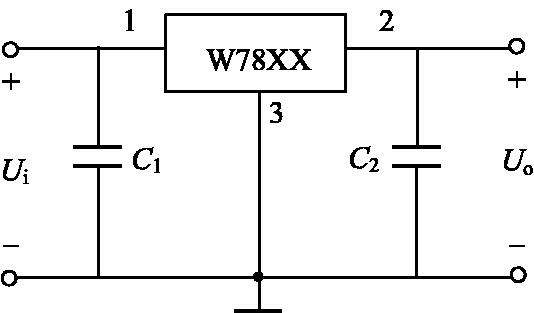
\includegraphics[width=0.35\textwidth]{集成稳压基本电路.jpg}
	\caption{集成稳压基本电路}
	\label{fig:集成稳压基本电路}
\end{figure}
\Par 如图\ref{fig:集成稳压基本电路}所示,它是集成稳压基本电路,左边的电容用于抵消输入端较长接线的电感效应,防止产生自激振荡;右边的电容用于防止瞬时增减负载电流,不致引起输出电压有较大的波动.

\begin{figure}[htbp]
	\centering
	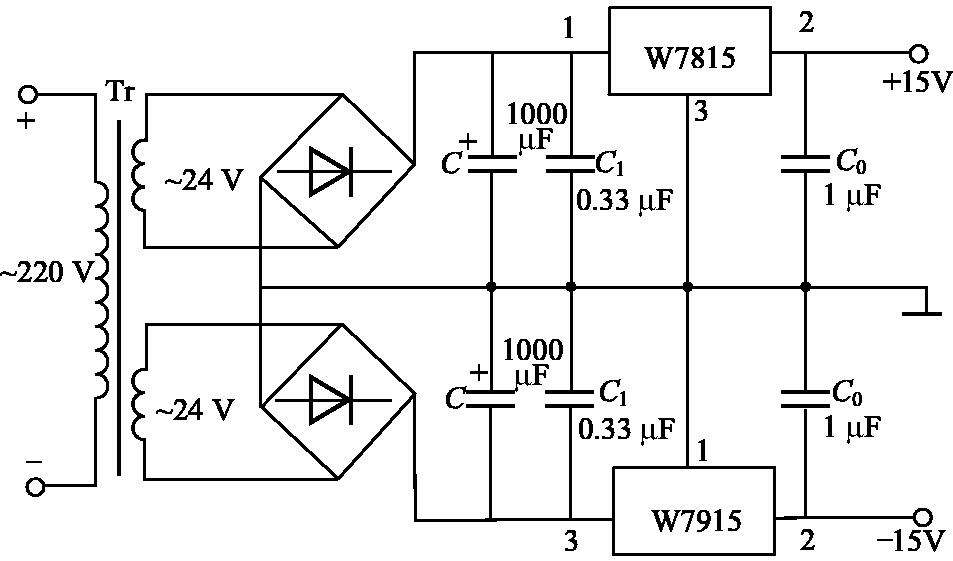
\includegraphics[width=0.65\textwidth]{正负输出稳压电路.jpg}
	\caption{正负输出稳压电路}
	\label{fig:正负输出稳压电路}
\end{figure}

\Par 如图\ref{fig:正负输出稳压电路}所示,这是一个正负输出稳压电路,分析上面的W7815稳压电源:首先,220V交流电源经过变压器转换成24V的交流电,经过单相桥式整流电路,将交流电转换成直流电并经过电桥滤波电路,接到集成稳压电源W7815的接口1.

\Par 这里W7815的“15”表示输出电压是15V,W78XX就表示输出电压是XXV.

\Par 接到集成稳压电源W7815的接口1后,我们可以注意到它的接口3接地,接口2输出15V的稳压直流电,因此我们可以判断它是金属封装.

\Par 对于集成稳压电源W7915也是同样,通过观察,我们知道它接口3输入,接口1接地,接口2输出,因此它也是金属封装.由于W7915输出的是负电压,因此它输出$-15$V电压.

\Par 那么W78XX/W79XX系列真的完全不能调整电压吗,当然可以,只是需要魔改.试看下面的电路:
\begin{figure}[htbp]
	\centering
	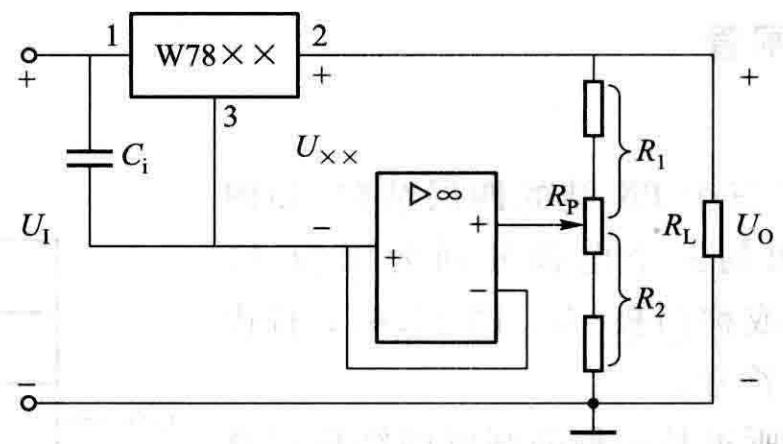
\includegraphics[width=0.45\textwidth]{电压可调稳压电路.png}
	\caption{电压可调稳压电路}
	\label{fig:电压可调稳压电路}
\end{figure}

我们可以发现它应当是金属封装W78XX系列,接口2、3之间的电压是$U_{XX}$,同时接口3与集成运算放大器的输出端相连,集成运算放大器工作在线性区,根据我们之前的讨论可以知道它具有\textbf{虚断}和\textbf{虚短}的特性.那么,集成运算放大器的负向输入端电位就与接口3的电位V$_3$相等,而根据虚短原则,可以知道正向输入端的电位也应当是V$_3$,那么根据分压原理就有
\begin{equation}
    U_{XX}=U_2=\frac{R_2}{R_1+R_2}U_O\Longrightarrow U_O=\left( 1+\frac{R_1}{R_2} \right) U_{XX}
\end{equation}

